\documentclass[tikz]{standalone}
\usepackage{pgfplots}
\pgfplotsset{compat=1.15}
\usepackage{mathrsfs}
\usetikzlibrary{arrows,calc}
\usepackage{tkz-euclide}
\pagestyle{empty}

\definecolor{AngleClr}{rgb}{0,0.39215686274509803,0}
\definecolor{ShapeClr}{rgb}{0.6,0.2,0}

\begin{document}

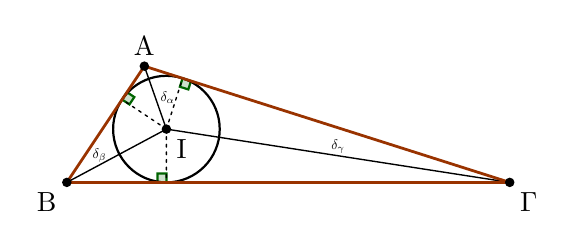
\begin{tikzpicture}[scale=.75]
\tkzSetUpLine[line width=1pt,color=black]
\tkzSetUpPoint[fill=black]

% \tkzDefPoints{0/0/A,7.5/0/B,1.3125/2.15625/C}
\tkzDefPoints{0/0/B,7.5/0/C,1.3125/1.96875/A}

\tkzInCenter(A,B,C)\tkzGetPoint{I}
\tkzDefPointBy[projection=onto A--B](I)\tkzGetPoint{IC}
\tkzDefPointBy[projection=onto B--C](I)\tkzGetPoint{IA}
\tkzDefPointBy[projection=onto A--C](I)\tkzGetPoint{IB}

\tkzFillPolygon[fill=white](A,B,C)

\tkzMarkRightAngles[line width=0.8pt, size=.15,color=AngleClr,fill=AngleClr,fill opacity=0.2](I,IC,A I,IB,C I,IA,B)

\tkzDrawSegments[line width=0.5pt,color=black,dashed,dash pattern=on 1pt off 1.75pt](I,IA I,IB I,IC)

\tkzDrawSegments[line width=0.5pt,color=black](A,I B,I C,I)

\tkzDrawCircle[line width=0.8pt, black](I,IA)


\tkzDrawPolygon[color=ShapeClr](A,B,C)
\tkzDrawPoints[size=3](A,B,C,I)
\tkzLabelPoint[above](A){$\rm A$}
\tkzLabelPoint[below left](B){$\rm B$}
\tkzLabelPoint[below right](C){$\rm \Gamma$}
\tkzLabelPoint[below right](I){$\rm I$}

\tkzLabelSegment[right,scale=0.5,pos=0.5](A,I){$\delta_\alpha$}
\tkzLabelSegment[left](B,I){\scalebox{0.5}{$\delta_\beta$}}
\tkzLabelSegment[above=-0.1cm](C,I){\scalebox{0.5}{$\delta_\gamma$}}

\end{tikzpicture}

\end{document}
